\section{虚继承}
\textbf{虚继承(Virtual inheritance)}用于对症解决菱形继承关系中公共基类重复的问题。如果两个基类虚继承自同一个公共基类,那么当其它类继承这两个类时,其公共基类部分的内容只会保留单独的一份,如图10.8所示。\par
\begin{figure}[htbp]
    \centering
    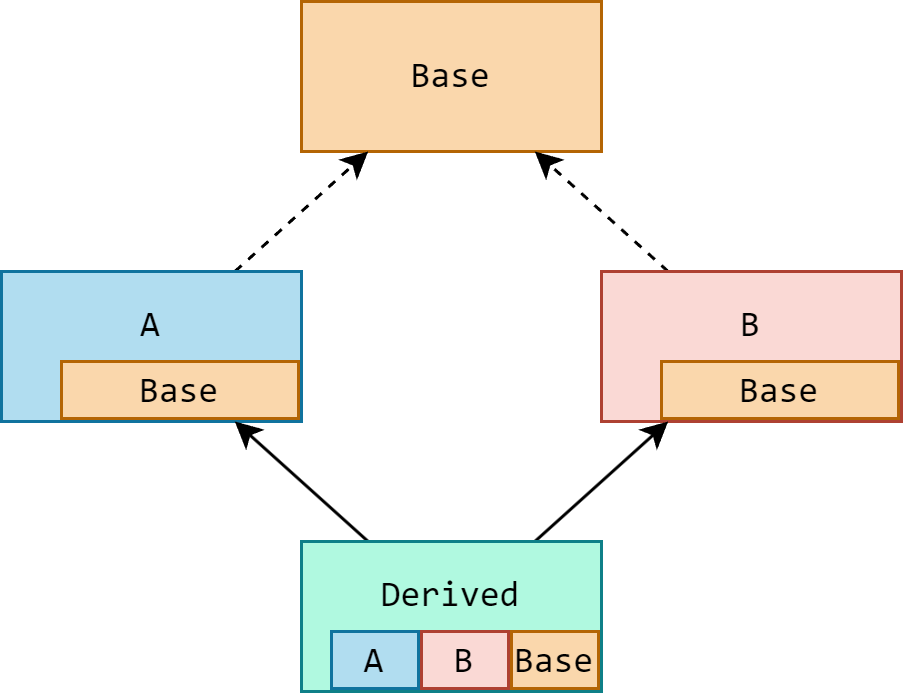
\includegraphics[width=.56\textwidth]{../images/generalized_parts/10_diamond_virtual_inheritance_300.png}
    \caption{虚继承的情况下,\lstinline@Derived@ 类只含有一份 \lstinline@Base@ 类对象}
\end{figure}
请读者务必注意虚继承使用的位置。不是 \lstinline@Derived@ 虚继承了 \lstinline@A@ 和 \lstinline@B@,而是 \lstinline@A@ 和 \lstinline@B@ 虚继承了 \lstinline@Base@。
如果要用代码来展现,只需要在继承 \lstinline@Base@ 时在前面添加一个 \lstinline@virtual@ 关键字即可。
\begin{lstlisting}
struct Base { int num {0}; };
struct A : virtual Base {}; //A类虚继承自Base
struct B : virtual Base {}; //B类虚继承自Base
struct Derived : A, B {}; //Derived类不需要虚继承自A或B
int main() {
    Derived de;
    std::cout << &de.A::num << std::endl << &de.B::num;
    //de的A::num成员和B::num成员是同一成员吗?地址值能告诉我们答案
}
\end{lstlisting}
这段代码的运行结果是:\\\noindent\rule{\linewidth}{.2pt}\texttt{
0x7ffce53da590\\
0x7ffce53da590
}\\\noindent\rule{\linewidth}{.2pt}
运行结果表明,这两个成员是相同的。\par
\subsection*{虚基类的初始化}
进行了虚继承的基类 \lstinline@Base@ 可以叫作虚基类(Virtual base class)\footnote{笔者本人十分反对使用``虚基类''这个名字。笔者认为,虚继承乃是继承操作的属性,与基类无关。如果部分派生类虚继承自 \lstinline@Base@ 而部分派生类没有虚继承自 \lstinline@Base@ 的话,这时候它究竟是不是虚基类,就说不清楚了。详见精讲篇。}。正如图10.8所示,在 \lstinline@Derived@ 类中,\lstinline@Base@ 既不是 \lstinline@A@ 的一部分,也不是 \lstinline@B@ 的一部分,而是单独的一部分。因此,在进行初始化时,虚基类的构造函数必须单独置于 \lstinline@Derived@ 类的初值列中。
\begin{lstlisting}
struct Base {
    Base (int i) : num {i} { //Base的构造函数
        std::cout << "Base::Base()\n";
    }
    int num;
};
struct A : virtual Base { //A类虚继承自Base
    A(int i, double d) : Base {i}, val {d} {
        std::cout << "A::A()\n";
    }
    double val;
};
struct B : virtual Base { //B类虚继承自Base
    B(int i, double d) : Base {i}, val {d} {
        std::cout << "B::B()\n";
    }
    double val;
};
struct Derived : A, B { //Derived类中有:Base::num, A::val, B::val
    Derived(int i, double d1, double d2)
        : Base {i}, A {i+1,d1}, B {i+2,d2}
    {
        std::cout << "Derived::Derived()\n";
    }
};
int main() {
    Derived d {0, .1, .2};
    std::cout << d.num << ' ' << d.A::val << ' ' << d.B::val;
}
\end{lstlisting}
这段代码的运行结果是\\\noindent\rule{\linewidth}{.2pt}\texttt{
Base::Base()\\
A::A()\\
B::B()\\
Derived::Derived()\\
0 0.1 0.2
}\\\noindent\rule{\linewidth}{.2pt}\par
在 \lstinline@Derived@ 的初值列中,虚基类 \lstinline@Base@ 的构造函数会被单独调用。而在调用 \lstinline@A@ 和 \lstinline@B@ 的构造函数时,它们初值列中调用 \lstinline@Base@ 的操作会被跳过——正因如此,我们才能看到 \lstinline@0@ 这个输出,而不是 \lstinline@1@ 或 \lstinline@2@(我们在 \lstinline@Derived@ 的构造函数中分别向 \lstinline@A::A(int,double)@ 和 \lstinline@B::B(int,double)@ 传递了 \lstinline@i+1@ 和 \lstinline@i+2@)。\par
总而言之,虚继承机制保证了虚基类 \lstinline@Base@ 的构造函数只被调用一次,这次调用是交给 \lstinline@Derived@ 直接进行的。\par
\subsection*{实操:平行四边形、菱形、矩形与正方形}
平行四边形是两组对边平行且相等的四边形;菱形是各边相等的平行四边形;矩形是内角为$90^\circ$的平行四边形;正方形是内角为$90^\circ$的菱形,或者说各边相等的矩形。从这个关系中我们不难看出,正方形是一种很特殊的平行四边形,它既有菱形的特征,又有矩形的特征。这非常符合多重继承的要求:正方形是一种菱形;正方形也是一种矩形。\par
描述一个平行四边形至少需要两条边,一个角;描述一个菱形至少需要一条边,一个角;描述一个矩形至少需要两条边;描述一个正方形最简单,至少需要一条边。所以它们之间也存在着
``基类比派生类更复杂''的情况,需要用抽象基类的方式来建立继承结构,见图10.9。\par
\begin{figure}[htbp]
    \centering
    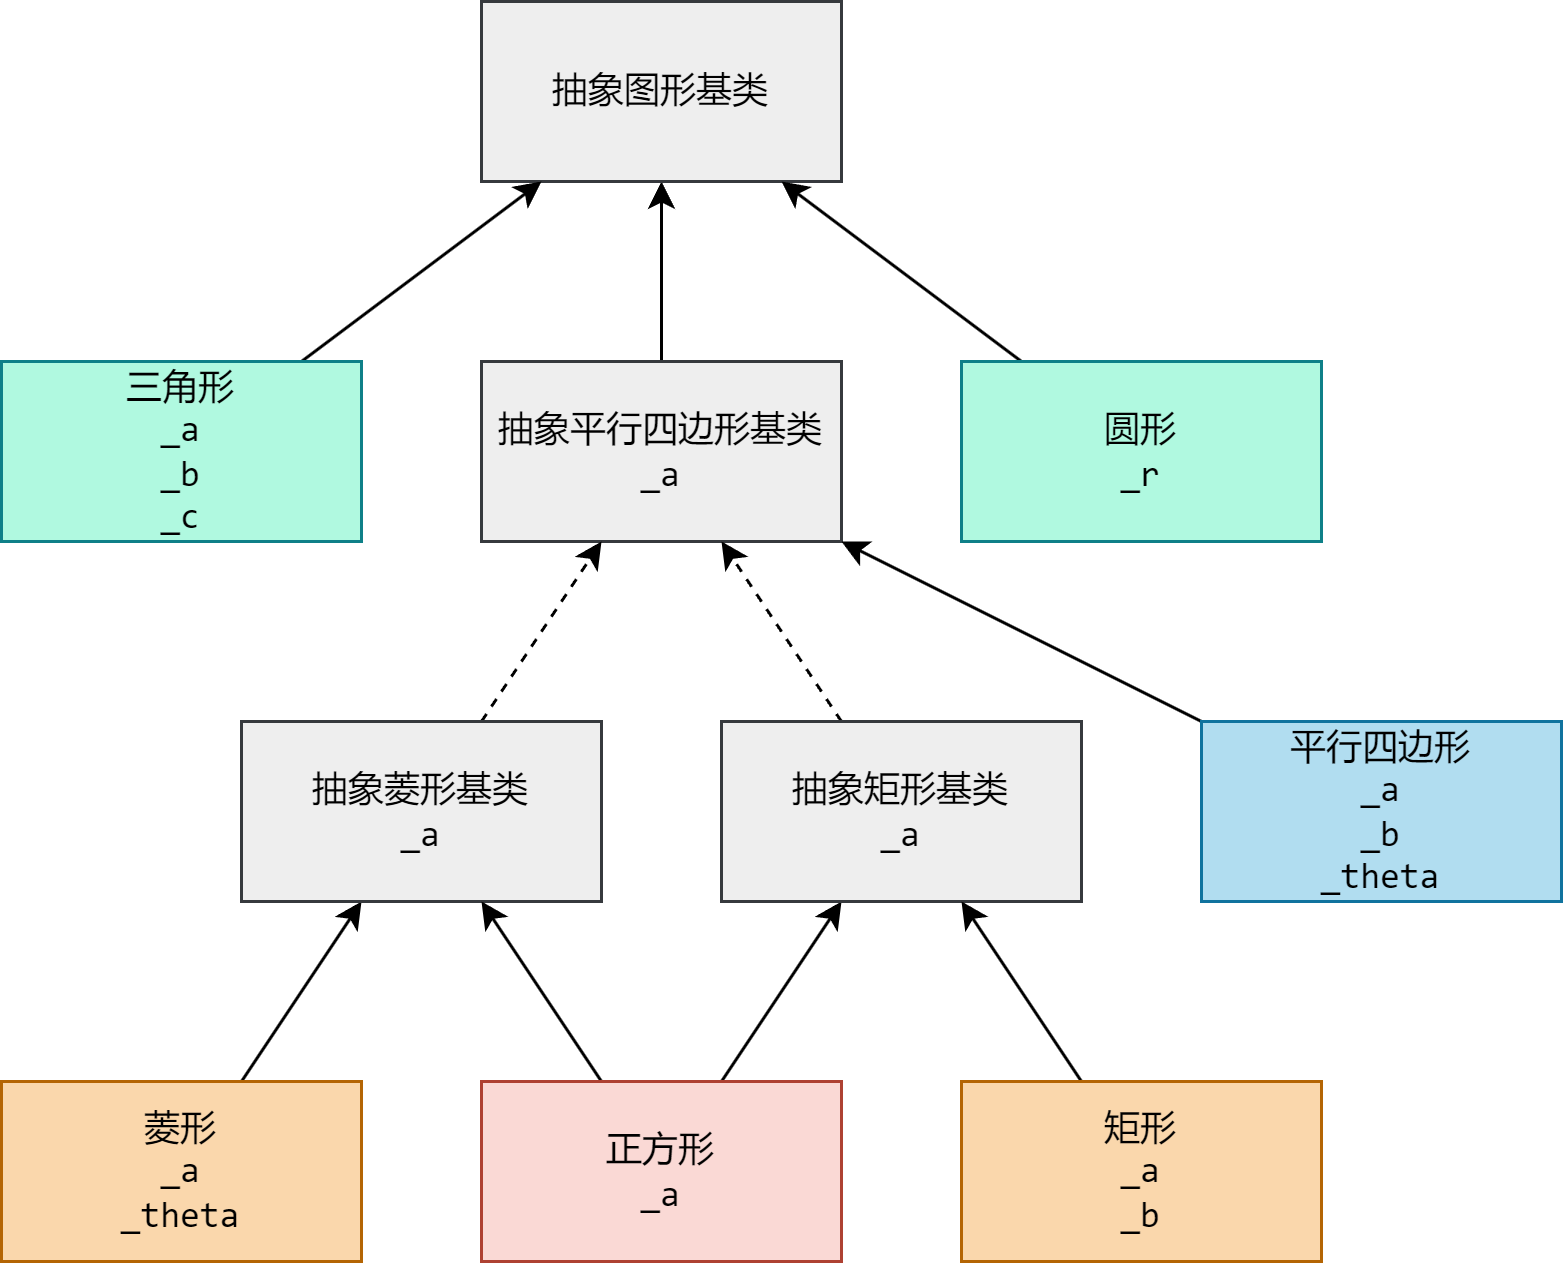
\includegraphics[width=.7\textwidth]{../images/generalized_parts/10_abstract_shape_class_with_multiple_inheritance_300.png}
    \caption{从 \lstinline@Shape@ 到各个图形之间的继承关系}
\end{figure}
其中的三角形、圆形之类,我们已经在第三节中完成了,所以这里从抽象平行四边形基类开始重写就好。
\begin{lstlisting}
//这些内容不变,原封不动复制下来就好
class Parallelogram_abc : public Shape { // 抽象平行四边形基类
protected:
    double _a; //所有平行四边形都至少需要一条边长信息
public:
    Parallelogram_abc(double a) : _a {a} {} //构造函数
};
class Parallelogram : public Parallelogram_abc { //平行四边形
    double _b;
    double _theta;
public:
    Parallelogram(double a, double b, double theta)
        : Parallelogram_abc {a}, _b {b}, _theta {theta} {}
    double perimeter()const { return 2 * (_a + _b); }
    double area()const { return _a * _b * std::sin(Deg2Rad(_theta)); }
};
\end{lstlisting}\par
抽象菱形基类和抽象矩形基类都是正方形的基类。所以为了避免成员的重复,我们需要让它们虚继承自抽象平行四边形基类。
\begin{lstlisting}
struct Rhombus_abc : virtual public Parallelogram_abc { //抽象菱形基类
    Rhombus_abc(double a) : Parallelogram_abc {a} {}
    double perimeter()const { return 4 * _a; } //菱形、正方形通用的周长公式
};
struct Rectangle_abc : virtual public Parallelogram_abc { //抽象矩形基类
    Rectangle_abc(double a) : Parallelogram_abc {a} {}
};
\end{lstlisting}\par
至于菱形和矩形,需要读者注意的是,因为 \lstinline@Rhombus_abc@ 虚继承自 \lstinline@Parallelogram_abc@,所以我们在 \lstinline@Rhombus@ 派生类的初值列中必须也要调用 \lstinline@Parallelogram_abc@ 的构造函数。
\begin{lstlisting}
    class Rhombus : public Rhombus_abc { //菱形
    double _theta;
public:
    Rhombus(double a, double theta)
        : Parallelogram_abc {a}, Rhombus_abc {a}, _theta {theta} {}
    //因为Rhombus_abc虚继承自Parallelogram_abc,我们必须单独调用后者的构造函数
    //又因为Rhombus继承自Rhombus_abc,我们必须调用后者的构造函数
    double area()const { return _a * _a * std::sin(Deg2Rad(_theta)); }
};
class Rectangle : public Rectangle_abc { //矩形
    double _b;
public:
    Rectangle(double a, double b)
        : Parallelogram_abc {a}, Rectangle_abc {a}, _b {b} {}
    //同上,不再赘述
    double perimeter()const { return 2 * (_a + _b); }
    double area()const { return _a * _b; }
};
\end{lstlisting}\par
最后只需要把正方形写出来就可以了。它多重继承自 \lstinline@Rhombus_abc@ 和 \lstinline@Rectangle_abc@,而它们又虚继承自 \lstinline@Parallelogram_abc@,所以我们要把这三个构造函数都写在 \lstinline@Square@ 类的初值列中。
\begin{lstlisting}
struct Square : Rhombus_abc, Rectangle_abc { //正方形
    Square(double a)
        : Parallelogram_abc {a}, Rhombus_abc {a}, Rectangle_abc {a} {}
    double area()const { return _a * _a; }
    //perimeter函数继承自Rhombus_abc足矣,不必再写
};
\end{lstlisting}\par
\subsection*{初学者对虚继承的常见困惑}
{\kaishu 虚继承和虚函数都用 \lstinline@virtual@ 关键字来实现,它们之间有什么关系吗?}\par
答案是,没有任何关系——或者说,本来是没有任何关系的。虚函数的目的是为了实现多态,即,可以用基类的指针调用派生类的成员函数;虚继承的目的是为了在菱形继承关系中保留单一的公共基类成员。它们的使用场合相互独立,完全无关。\par
至于它们都用 \lstinline@virtual@ 关键字来实现,这可以理解成是语言中的``一词多义''。这种一词多义的现象不仅存在于自然语言\footnote{自然语言(Natural language)指的是自然地产生于人类社会中,并随着人类的使用及社会的发展而不断演变的语言,比如汉语,英语等;与之相对的是世界语等人工语言,以及编程语言等形式语言。}中,也普遍存在于编程语言中。一个运算符 \lstinline@*@,当它接收两个操作数时就意味着乘法运算;当它接收一个操作数时就意味着取内容运算。\par
C++标准对于关键字的引入是很``吝啬''的。因此如果要实现什么新功能的话,一般会优先选择已有的关键字。比如说C++11标准把 \lstinline@auto@ 的用途改换成了自动类型推导说明符,还为 \lstinline@delete@ 关键字添加了弃置函数功能。\par
至于为什么要用虚继承这个名字,斯特劳斯特鲁普在他的《C++语言的设计与演化》\footnote{\textit{The Design and Evolution of C++}.}一书中也有所解释,读者可以自行查阅。\par
{\kaishu 虚继承可以用来解决多重继承中的名称冲突问题吗?}\par
这个问题的答案是``不''。虚继承根本就不是为了解决名称冲突而提供的机制,它存在的作用是保证共同基类中的内容不重复。
\begin{lstlisting}
struct Base {};
struct A : virtual Base { int num; };
struct B : virtual Base { double num; };
struct Derived : virtual A, virtual B {};
int main() {
    Derived d;
    std::cout << &d.A::num << '\n' << &d.B::num; //会输出不一样的结果
}
\end{lstlisting}\par
{\kaishu 虚继承能像虚函数那样向下传递吗?}\par
虚继承这个``关系''不会向下传递。这也就意味着,虽然 \lstinline@A@ 和 \lstinline@B@ 虚继承自 \lstinline@Base@,但是 \lstinline@Derived@ 与 \lstinline@A@ 或 \lstinline@B@ 之间也未必是虚继承关系。如果我们希望 \lstinline@Derived@ 虚继承自 \lstinline@A@ 或 \lstinline@B@,那么我们必须像上面的代码中那样,都写上 \lstinline@virtual@ 才行。\par
但是虚继承这条``信息''可以向下传递。对于 \lstinline@Base@ 的所有间接派生类(无论这个派生类是否直接或间接地进行了多重继承)来说,\lstinline@Base@ 始终是独立于 \lstinline@A@ 和 \lstinline@B@ 等内嵌对象而存在的——它们只有名义上的派生关系,而在构造、初始化等方面表现得更像是并列关系。\par
以前述代码中的 \lstinline@Rhombus@ 类为例吧,虽然它从未参与过多重继承,但是既然 \lstinline@Rhombus_abc@ 与 \lstinline@Parallelogram_abc@ 是虚继承关系,那么 \lstinline@Rhombus@ 的构造函数就必须把 \lstinline@Parallelogram_abc@ 当成一个独立的对象来看待。所以我们就能看到,\lstinline@Rhombus::Rhombus()@ 的初值列中调用了两个基类构造函数,一个属于直接基类 \lstinline@Rhombus_abc@,一个属于虚基类 \lstinline@Parallelogram_abc@。\par
\begin{lstlisting}
    Rhombus(double a, double theta)
        : Parallelogram_abc {a}, Rhombus_abc {a}, _theta {theta} {}
    //因为Rhombus_abc虚继承自Parallelogram_abc,我们必须单独调用后者的构造函数
    //又因为Rhombus继承自Rhombus_abc,我们必须调用后者的构造函数
\end{lstlisting}\par
如果 \lstinline@Rhombus@ 还有自己的派生类,那么这个派生类的初值列中需要调用两个函数,一个属于直接基类 \lstinline@Rhombus@,还有一个属于虚基类 \lstinline@Parallelogram_abc@。至于 \lstinline@Rhombus_abc@,它不是 \lstinline@Rhombus@ 的虚基类,所以不能视作一个独立的对象来看待,它是内嵌于 \lstinline@Rhombus@ 当中的。这同样能说明虚继承这一关系不可向下传递,而虚继承这则信息能一直向下传递。\par
{\kaishu 如果有些类虚继承自 \lstinline@Base@ 而有些类不是虚继承自 \lstinline@Base@,那会怎么样?}\par
虚继承的那些类会共享同一个虚基类,而非虚继承的那些类会各有一份内嵌的基类。我举个例子你就懂了:
\begin{lstlisting}
struct Base { int num {0}; };
struct A : virtual Base {}; //A类虚继承自Base
struct B : virtual Base {}; //B类虚继承自Base
struct C : Base {}; //C类非虚继承自Base
struct D : Base {}; //D类非虚继承自Base
struct Derived : A, B, C, D {};
int main() {
    Derived de;
    std::cout
        << &de.A::num << std::endl
        << &de.B::num << std::endl
        << &de.C::num << std::endl
        << &de.D::num << std::endl;
    //有几个num成员呢?地址值会告诉我们答案
}
\end{lstlisting}
这段代码的运行结果如下:\\\noindent\rule{\linewidth}{.2pt}\texttt{
0x7ffc3f7480b8\\
0x7ffc3f7480b8\\
0x7ffc3f7480b0\\
0x7ffc3f7480b4
}\\\noindent\rule{\linewidth}{.2pt}
我们看到,\lstinline@d.A::num@ 和 \lstinline@d.B::num@ 是同一个成员。而 \lstinline@d.C::num@ 和 \lstinline@d.D::num@ 各自对应着一个成员。所以 \lstinline@Derived@ 类总共有三个不同的 \lstinline@num@ 成员。\par
\subsection*{有关几何图形的完整代码}
代码10.1是有关几何图形问题的完整代码。因为所有内容都是在类内定义的,所以只需要一个头文件就足够了。\par
这段代码中包含了虚函数、抽象基类、多重继承和虚继承的相关知识,读者可以对照注释内容尝试理解。我相信以读者现在的水平,是可以看懂这些代码的。\par
如果难以理解某处的继承关系,记得回去看图10.9。一图胜千言。\par
\lstinputlisting[caption=\texttt{Header.hpp}]{code_in_book/10.1/Header.hpp}
